\documentclass[]{article}
\usepackage{graphicx}
\usepackage[svgnames]{xcolor} 
\usepackage{fancyhdr}
\usepackage{tocloft}
\usepackage[hidelinks]{hyperref}
\usepackage{enumitem}
\usepackage[many]{tcolorbox}
\usepackage{listings }
%\usepackage[a4paper, total={6in, 8in} , top = 2cm,bottom = 4cm]{geometry}
\usepackage[a4paper, total={6in, 8in}]{geometry}
\usepackage{afterpage}
\usepackage{amssymb}
\usepackage{hyperref}
\usepackage{pdflscape}
\usepackage{textcomp}
\usepackage{xecolor}
\usepackage{rotating}
\usepackage{xepersian}
\usepackage[T1]{fontenc}
\usepackage{tikz}
\usepackage[utf8]{inputenc}
\usepackage{PTSerif} 
\usepackage{seqsplit}
\usepackage{changepage}


\usepackage{listings}
\usepackage{xcolor}
\usepackage{sectsty}

\setcounter{secnumdepth}{0}
 
\definecolor{codegreen}{rgb}{0,0.6,0}
\definecolor{codegray}{rgb}{0.5,0.5,0.5}
\definecolor{codepurple}{rgb}{0.58,0,0.82}
\definecolor{backcolour}{rgb}{0.95,0.95,0.92}
\definecolor{blanchedalmond}{rgb}{1.0, 0.92, 0.8}
\definecolor{brilliantlavender}{rgb}{0.96, 0.73, 1.0}
 
\NewDocumentCommand{\codeword}{v}{
\texttt{\textcolor{blue}{#1}}
}
\lstset{language=java,keywordstyle={\bfseries \color{blue}}}

\lstdefinestyle{mystyle}{
    backgroundcolor=\color{backcolour},   
    commentstyle=\color{codegreen},
    keywordstyle=\color{magenta},
    numberstyle=\tiny\color{codegray},
    stringstyle=\color{codepurple},
    basicstyle=\ttfamily\normalsize,
    breakatwhitespace=false,         
    breaklines=true,                 
    captionpos=b,                    
    keepspaces=true,                 
    numbers=left,                    
    numbersep=5pt,                  
    showspaces=false,                
    showstringspaces=false,
    showtabs=false,                  
    tabsize=2
}

\lstset{style=mystyle}

 \settextfont[BoldFont={XB Zar bold.ttf}]{XB Zar.ttf}


\setlatintextfont[Scale=1.0,
 BoldFont={LiberationSerif-Bold.ttf}, 
 ItalicFont={LiberationSerif-Italic.ttf}]{LiberationSerif-Regular.ttf}





\newcommand{\inputsample}[1]{
    ~\\
    \textbf{ورودی نمونه}
    ~\\
    \begin{tcolorbox}[breakable,boxrule=0pt]
        \begin{latin}
            \large{
                #1
            }
        \end{latin}
    \end{tcolorbox}
}

\newcommand{\outputsample}[1]{
    ~\\
    \textbf{خروجی نمونه}

    \begin{tcolorbox}[breakable,boxrule=0pt]
        \begin{latin}
            \large{
                #1
            }
        \end{latin}
    \end{tcolorbox}
}

\newtcolorbox{mybox}[2][]{colback=red!5!white,
colframe=red!75!black,fonttitle=\bfseries,
colbacktitle=red!85!black,enhanced,
attach boxed title to top center={yshift=-2mm},
title=#2,#1}

\newenvironment{changemargin}[2]{%
\begin{list}{}{%
\setlength{\topsep}{0pt}%
\setlength{\leftmargin}{#1}%
\setlength{\rightmargin}{#2}%
\setlength{\listparindent}{\parindent}%
\setlength{\itemindent}{\parindent}%
\setlength{\parsep}{\parskip}%
}%
\item[]}{\end{list}}


\definecolor{foldercolor}{RGB}{124,166,198}
\definecolor{sectionColor}{HTML}{ff5e0e}
\definecolor{subsectionColor}{HTML}{008575}

\definecolor{listColor}{HTML}{00d3b9}

\definecolor{umlrelcolor}{HTML}{3c78d8}

\definecolor{subsubsectionColor}{HTML}{3c78d8}

\definecolor{CustomColor}{HTML}{A61C00}


\defpersianfont\authorFont[Scale=0.9]{XB Zar bold.ttf}

\defpersianfont\titr[Scale=1.5]{Lalezar-Regular.ttf}

\defpersianfont\fehrest[Scale=1.2]{Lalezar-Regular.ttf}

\defpersianfont\fehrestTitle[Scale=3.0]{Lalezar-Regular.ttf}

\defpersianfont\fehrestContent[Scale=1.2]{XB Zar bold.ttf}


\sectionfont{\color{sectionColor}}  % sets colour of sections
\subsectionfont{\color{subsectionColor}}  % sets colour of sections
\subsubsectionfont{\color{subsubsectionColor}}


\renewcommand{\labelitemii}{$\circ$}


\renewcommand{\baselinestretch}{1.1}


\renewcommand{\contentsname}{فهرست}

\renewcommand{\cfttoctitlefont}{\fehrestTitle}


\renewcommand\cftsecfont{\color{sectionColor}\fehrestContent\selectfont}
\renewcommand\cftsubsecfont{\color{subsectionColor}\fehrestContent\selectfont}
\renewcommand\cftsubsubsecfont{\color{subsubsectionColor}\fehrestContent\selectfont}
%\renewcommand{\cftsecpagefont}{\color{sectionColor}}

\setlength{\parskip}{1.2pt}

\begin{document}


%%% title pages
\begin{titlepage}
\begin{center}

\textbf{ \Huge{به نام خدا} }
        
\vspace{0.2cm}


\includegraphics[width=0.4\textwidth]{Logo/aut-fa2.png}\\
\vspace{0.2cm}
\textbf{ \Huge{\emph درس مدار‌های منطقی} }\\
\vspace{0.25cm}
\textbf{ \Large{ پروژه نهایی} }
\vspace{0.2cm}
       
 
      \large \textbf{دانشکده مهندسی کامپیوتر}\\\vspace{0.1cm}
    \large   دانشگاه صنعتی امیرکبیر\\\vspace{0.2cm}
       \large   ﻧﯿﻢ سال دوم ۰۳-۰۲ \\\vspace{0.10cm}
      \noindent\rule[1ex]{\linewidth}{1pt}
استاد:\\
    \textbf{{دکتر مرتضی صاحب‌الزمانی}}



    \vspace{0.20cm}

   مهلت ارسال و ارائه:\\
    \textbf{{17 تیر}}

    \vspace{0.10cm}
مسئول پروژه:\\
    \textbf{\authorFont{مدرسین آزمایشگاه منطقی}}
    
        \vspace{0.10cm}
طراحان پروژه:\\
    \textbf{\authorFont{ رضا آدینه پور، محمد مهدی نعمتی }}
    

\end{center}
\end{titlepage}
%%% title pages


%%% header of pages
\newpage
\pagestyle{fancy}
\fancyhf{}
\fancyfoot{}
\cfoot{\thepage}
\lhead{نیمسال ۰۳-۰۲}
\rhead{
\includegraphics[width=0.1\textwidth]{Logo/ce-fa.png}\\
دانشکده مهندسی کامپیوتر
}
\chead{پروژه مدارمنطقی}
%%% header of pages
\renewcommand{\headrulewidth}{2pt}



\tableofcontents

\newpage

 \Large \textbf{\\
}

\section*{{\titr نکات قابل توجه}}
\addcontentsline{toc}{section}{{\fehrestContent نکات قابل توجه}}
\begin{itemize}
	
\item 
ددلاین تحویل فاز اول پروژه، در روز‌های \textbf{شنبه، ۱۹} و \textbf{دوشنبه، ۲۱ خرداد}\footnote{هر گروه در زمان کلاس خودش} در کلاس آزمایشگاه است. همچنین تحویل فاز دوم پروژه، \textbf{یکشنبه ۱۷ تیر} خواهد بود.
	
\item
انجام پروژه به‌صورت گروهی‌ست و گروه‌های شما همان گروه‌های آزمایشگاه است. درصورت وجود مشکل موجه، با هماهنگی با مدرسین آزمایشگاه می‌توانید گروه خود را تغییر دهید.


\item
دانشجویان \textbf{ملزم به تحویل حضوری} هر دو فاز پروژه هستند. درصورتی که گروهی در روز تحویل حاضر نشود نمره‌ای به ایشان تعلق نخواهد گرفت.

\item
در روز تحویل حضوری مشارکت تمام اعضای تیم در پروژه بررسی خواهد‌ شد و در صورت عدم مشارکت بعضی از اعضا، نمرهٔ ایشان برای آن فاز از پروژه "صفر" لحاظ می‌گردد. مشارکت، با توجه به commit های افراد تیم در مخزن گیت‌هاب پروژه و سوالات پرسیده شده در روز تحویل و با صلاحدید مدرس مشخص می‌شود.

\item
ددلاین فاز اول و دوم در آخرین زمان ممکن قبل از تحویل نمرات قرار داده شده است. لذا در هر دو فاز \textbf{مهلت تاخیر وجود ندارد}.

\item
در صورت کشف تقلب از هریک از تیم‌ها، برای بار اول منفی نمرهٔ آن فاز برای آن تیم ثبت می‌شود و برای بار دوم، نمرهٔ منفی کل پروژه برای تیم لحاظ خواهد‌ شد که معادل \textbf{مردود شدن} در درس است.
\end{itemize}

\newpage



 \Large \textbf{\\
}

\section*{{\titr مقدمه}}
\addcontentsline{toc}{section}{{\fehrestContent مقدمه}}


\subsection*{{\titr یعقوب\footnote{\lr{Electronic Jacob}} برقی که بود؟}}
\addcontentsline{toc}{subsection}{{\fehrestContent یعقوب برقی که بود؟}}

\textbf{هر امیرکبیری میدونه!}

که اسم جهانی یعقوب برقی\footnote{برگرفته از یعقوب آقا، دکه وسط صحن دانشگاه} مخصوص دستگاه‌های فروش خودکار است که اگر با همین نام اون رو در گوگل سرچ کنید متوجه جهانی بودن این اسم می‌شوید.


\begin{figure}[h]
	\centering
	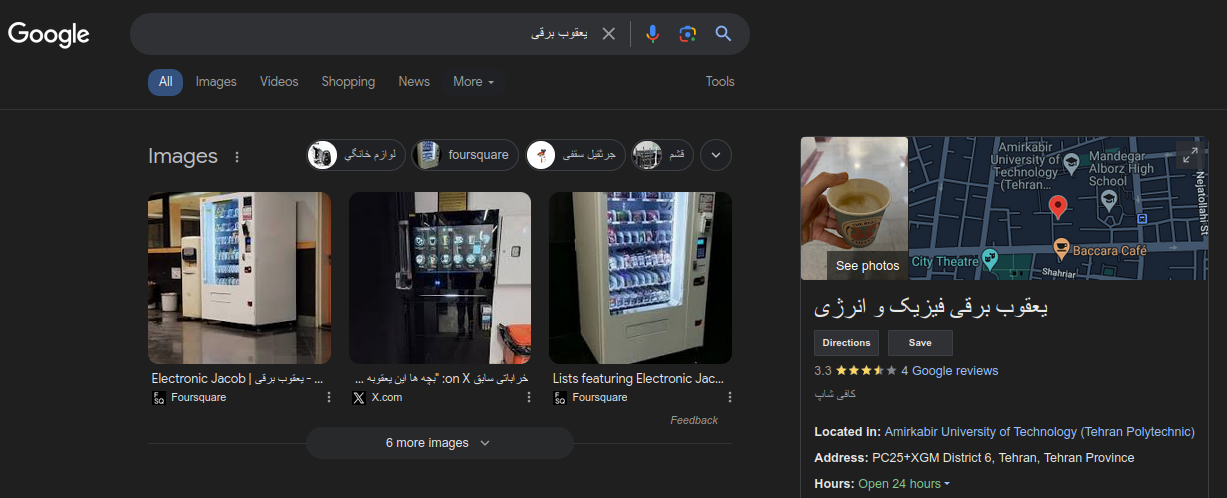
\includegraphics[width=1\textwidth]{images/img1}
	\caption{این نام جهانیست!}
	\label{این نام جهانیست!}
\end{figure}








احتمالا همگی یعقوب برقی دانشکده رو دیدین و از اون استفاده کردین.
%
%\begin{figure}[h]
%	\centering
%	
\includegraphics[width=0.5\textwidth]{images/img2}
%	\caption{یعقوب برقی}
%	\label{یعقوب برقی}
%\end{figure}

در این پروژه قصد داریم کمی بیشتر با یعقوب برقی آشنا بشیم و بخش کوچکی از سیستم کنترلی اون رو شبیه‌سازی کنیم.

بعد از انجام این پروژه، خرید‌های شما از یعقوب برقی، فقط یک خرید ساده نیست!




\Large \textbf{\\\\\\
}



\subsection*{{\titr فاز ۱}}
\addcontentsline{toc}{subsection}{{\fehrestContent فاز ۱}}
این پروژه در دو فاز انجام می‌شود. در فاز اول قراه پیش‌نیاز‌های مهمی از فاز دوم رو انجام بدید. تحویل فاز اول مهمه 




\subsection*{{\titr فاز ۲}}
\addcontentsline{toc}{subsection}{{\fehrestContent فاز ۲}}














\begin{itemize}


\item
 با مفاهیم شبکه آشنا می‌شوید و فروشگاه خود را با معماری کلاینت-سرور پیاده سازی می‌کنید.
 
 \item
 
به فروشگاه خود یک سری ویژگی‌ها اضافه می‌کنید. (از جمله بانک، مزایده و … )

\item
با یک سری مفاهیم (پیشرفته‌تر)‌ در برنامه نویسی آشنا می‌شوید. ( از جمله پایگاه‌داده، توکن، مفاهیم مربوط به امنیت، معماری \lr{P2P} و …)

\end{itemize}
\newpage



 \Large \textbf{\\
}
\section*{{\titr بخش‌های اصلی }}
\addcontentsline{toc}{section}{{\fehrestContent بخش‌های اصلی}}

\subsection*{{\titr شبکه چیست؟}}
\addcontentsline{toc}{subsection}{{\fehrestContent شبکه چیست؟}}

قبل از هر چیز نیاز داریم که نسبت به شبکه و مفاهیم آن شهود بدست بیاوریم. سپس با استفاده از این شهود ، ابزار‌ها و کتاب‌خانه‌های جاوا، بر بستر شبکه کد بزنیم. ( البته با توجه به تمرین شبکه، تا حدی با این مفاهیم کار کرده‌اید.)


برای آشنایی با شبکه و کد زدن، \textcolor{CustomColor}{داک شبکه} را مطالعه کنید.


در این فاز شما باید فروشگاه خود را به دو بخش کلاینت و سرور تقسیم کنید. سرور شما ابتدا اجرا می‌شود و یک تا چند کلاینت به آن متصل شده و با آن ارتباط برقرار می‌کنند ( کلاینت و سرور تنها از طریق شبکه با هم در ارتباط خواهند بود). با توجه به تعریف ها و مفاهیمی که از این معماری در داک بالا گفته شد، باید  بتوانید کلاس‌های مربوط سرور و کلاینت را تفکیک کنید.



\subsection*{{\titr بانک}}
\addcontentsline{toc}{subsection}{{\fehrestContent بانک}}

در این فاز به پروژه شما یک بانک افزوده می‌شود. این بانک به صورت یک سرور جدا ( از سرور و کلاینت فروشگاه‌) اجرا می‌شود. در داک زیر شیوه دقیق ارتباط با بانک ، واسط‌های کاربری  ( API )‌ و امکاناتی که در اختیار شما قرار می‌دهد گفته شده است. فایل اجرایی سرور این بانک بطور آماده به شما داده می‌شود(برای استخراج کد از این فایل تلاش نکنید)، اما پیاده سازی آن امتیازی است و امتیاز قابل توجهی نیز دارد. در صورتی که می‌خواهید بانک را خودتان پیاده سازی کنید، باید واسط‌های کاربریتان (API)‌ مطابق داک زیر باشد.

فایل اجرایی سرور بانکِ آماده ( به همراه یک نمونه کلاینت) در اختیار شما قرار می‌گیرد.

نحوه استفاده از بانک و API آن را می‌توانید در \textcolor{CustomColor}{داک بانک} مشاهده کنید.

\newpage


 \Large \textbf{\\
}
\subsection*{{\titr کیف پول}}
\addcontentsline{toc}{subsection}{{\fehrestContent کیف پول}}
در این فاز به \textcolor{CustomColor}{فروشگاه} شما، کیف پول اضافه می‌شود. به این شکل که برای هر حساب( فروشنده یا خریدار) یک کیف پول تعریف می‌شود که کاربر می‌تواند با استفاده از حساب بانکی خود(که به صورت جداگانه در بانک قرار دارد) آن را شارژ و یا از کیف پول خود مبلغی را برداشت کند. توجه کنید که خریدار برای خرید کردن باید حق انتخاب داشته باشد که مستقیما از حساب بانکی خود یا کیف پول خود خرید کند (مدیران فروشگاه حسابی مشترک در بانک تحت عنوان حساب فروشگاه دارند که تمامی اعتبار کیف پول‌های کاربران به درون آن ریخته می‌شود).


\begin{enumerate}

\item
خرید مستقیم با  استفاده از حساب بانکی: در صورت انتخاب این گزینه، مبلغ پرداختی از حساب کاربر (در بانک) به حساب فروشگاه (در بانک) انتقال می‌یابد (با استفاده از API بانک این کار انجام گیرد) و سپس کیف پول فروشنده با کسر کارمزد، شارژ‌ می‌شود.

\begin{itemize}[label=$\blacksquare$]
\item
مدیر باید بتواند کارمزد را تعیین کند. (مثلا 5 درصد)
\end{itemize}


\item
خرید با استفاده از اعتبار کیف پول:‌ در صورت انتخاب این گزینه، کل مبلغ از کیف پول خریدار کم شده و با کسر کارمزد، کیف پول فروشنده شارژ می‌شود.

\begin{itemize}[label=$\blacksquare$]
\item
مثلا اگر کارمزد ۵ درصد باشد، اگر خریدار کالایی با قیمت ۱۰۰ واحد بخرد، از کیف پولش ۱۰۰ واحد کم شده و به کیف پول فروشنده ۹۵ واحد اضافه می‌شود.
\end{itemize}

\end{enumerate}


هر فروشنده و خریدار باید بتواند بعد از login کردن عملیات زیر را با کیف پول خود انجام دهد:

\begin{enumerate}


\item
شارژ کیف پول

\item
برداشت از کیف پول

\begin{itemize}[label=$\blacksquare$]
\item
فقط فروشنده می‌تواند این کار را انجام دهد.

\item
همواره باید در کیف پول مقدار حداقلی باقی بماند که مدیر فروشگاه تعیین می‌کند.

\end{itemize}

\end{enumerate}



 \Large \textbf{\\
}
\subsection*{{\titr پشتیبانی}}
\addcontentsline{toc}{subsection}{{\fehrestContent پشتیبانی}}

در فروشگاه باید نقشی تحت عنوان پشتیبان داشته باشیم. ساخت اکانت پشتیبان همانند اکانت \textcolor{CustomColor}{مدیر} باید توسط مدیر انجام گیرد. سپس این افراد به حساب کاربری خود ورود می‌کنند (‌login).  هر خریدار می‌تواند از بین پشتیبان‌هایی که آنلاین هستند، یک نفر را انتخاب کرده و با او صحبت کند. پیاده سازی چت همزمان یک پشتیبان با چند خریدار، از موارد امتیازی است.

\subsection*{{\titr مزایده}}
\addcontentsline{toc}{subsection}{{\fehrestContent مزایده}}

یک فروشنده می‌تواند یکی از محصولاتش را برای مزایده بگذارد و زمانی را برای این مزایده تعیین کند که پس از آن، مزایده خاتمه یابد. 

\begin{enumerate}

\item
باید لیستی از مزایده‌ها برای خریداران وجود داشته باشد.

\item
خریدار با انتخاب یکی از مزایده‌ها وارد آن می شود و در ابتدا مبلغی را پیشنهاد می‌دهد که کمتر از شارژ کیف پولش است.

\item
خرید در مزایده تنها با کیف پول انجام می‌شود. (روال انتقال پول مثل خرید عادی است.)

\item
همه‌ی افراد شرکت کننده در مزایده، باید بتوانند با هم صحبت کنند. (چت چندنفره)

\item
خریدار تنها می‌تواند مبلغ پیشنهادی خود را افزایش دهد.


\end{enumerate}


\subsection*{{\titr خرید و فروش فایل}}
\addcontentsline{toc}{subsection}{{\fehrestContent خرید و فروش فایل}}

محصولی که فروشنده‌ها برای فروش می‌گذارند می‌تواند یک فایل باشد. در این صورت همانند محصولات عادی فروشنده آن را برای فروش می‌گذارد و آن را به سرور آپلود می‌کند، خریدار پس از خرید، آن را از سرور فروشگاه دانلود می‌کند.
 

 
در صورت پیاده سازی قسمت امتیازی P2P فرآیند انتقال فایل متفاوت است که در  \hyperref[subsec:p2p]{{\textcolor{blue}{\underline{انتها}}}} (\textcolor{CustomColor}{و داک \lr{P2P}}) توضیح داده شده است.

\subsection*{{\titr ارسال خرید}}
\addcontentsline{toc}{subsection}{{\fehrestContent ارسال خرید}}

بعد از خرید کردن توسط خریدار، باید لاگ خرید و آدرس خریدار در حساب مدیران فروشگاه قابل مشاهده باشد. مدیران باید بتوانند خرید‌های انجام شده را مشاهده کنند و وضعیت تحویل آن‌ها را به ارسال شده تغییر دهند. خریداران نیز در بخش تاریخچه خرید در حساب خود باید بتوانند وضعیت سفارش‌های خود را ببینند (‌ارسال شده یا در انتظار ارسال).

\begin{itemize}
\item
اگر محصول خریداری شده فایل بود، همین اطلاعات باید در حساب مدیران و خریداران قابل مشاهده باشد اما دیگر وضعیت ارسال و آدرس خریدار وجود نخواهد داشت.
\end{itemize}

\subsection*{{\titr توکن}}
\addcontentsline{toc}{subsection}{{\fehrestContent توکن}}

در محتوای مربوط به شبکه (داک شبکه)، توکن توضیح داده شد. پیاده سازی توکن برای ارتباط کاربران فروشگاه (‌با سرور فروشگاه)‌ نیز از موارد اجباری این فاز است.


\newpage


 \Large \textbf{\\
}
\section*{{\titr بخش‌های امتیازی}}
\addcontentsline{toc}{section}{{\fehrestContent بخش‌های امتیازی}}

از این قسمت به بعد وارد بخش‌های امتیازی پروژه می شویم. دقت کنید که این بخش های هم بسیار آموزنده و کاربردی هستند و هم می تواند به نمره پروژه شما به اندازه قابل توجهی اضافه کند. :)


\subsection*{{\titr وضعیت کاربران}}
\addcontentsline{toc}{subsection}{{\fehrestContent وضعیت کاربران}}

مدیران فروشگاه بتوانند وضعیت (‌آنلاین یا آفلاین) بودن کاربران را مشاهده کنند. به این صورت که لیستی از تمام کاربران و وضعیت آن‌ها وجود داشته باشد.

\subsection*{{\titr چت همزمان}}
\addcontentsline{toc}{subsection}{{\fehrestContent چت همزمان}}

همان طور که در بخش پشتیبان نیز گفته شد،‌ یک پشتیبان بتواند همزمان با چند خریدار صحبت کند.توجه کنید که باید فسمت گرافیکی این موضوع هم رعایت شود و پشتیبان بتواند به سهولت بین چت‌ها جابجا شود.


\subsection*{{\titr پایگاه داده}}
\addcontentsline{toc}{subsection}{{\fehrestContent پایگاه داده}}


برای ذخیره اطلاعات حساب‌ها در سرور، می توانید از پایگاه داده استفاده کنید (‌کاری که در برنامه‌های واقعی و عملی به جای ذخیره سازی خام در فایل انجام می شود).


برای این منظور در \textcolor{CustomColor}{داک پایگاه داده} مفاهیم مربوط به پایگاه داده و کار با آن در جاوا توضیح داده شد.



\subsection*{{\titr {REST}}}
\addcontentsline{toc}{subsection}{{\fehrestContent {REST}}}

برای ارتباط بین کلاینت و سرور،‌ می توانید از معماری نرم افزاری \lr{REST} استفاده کنید. \lr{REST} به عنوان عضوی از دنیای وب شناخته می‌شود و مزایا و کاربردهای بسیاری دارد. برای آشنایی و پیاده سازی آن به داک \lr{REST} مراجعه کنید.




\subsection*{{\titr بانک}}
\addcontentsline{toc}{subsection}{{\fehrestContent بانک}}

از موارد مهم امتیازی، پیاده سازی بانک است. شما می‌توانید بانک گفته شده را خودتان پیاده سازی کنید. دقت کنید که بانکی که شما پیاده می‌کنید باید API آن مشابه API بانک آماده‌ای که ما در اختیارتان قرار می‌دهیم باشد. (‌به دستورات گفته شده در
\textcolor{CustomColor}{داک بانک}
  مراجعه کنید)
 


\begin{itemize}[label = $\star$]
\item

در صورت مشابه بودن کد بانک شما به بانکی که ما در اختیارتان قرار می‌دهیم،‌ برای شما \textcolor{CustomColor}{تقلب} منظور می‌گردد.


\end{itemize}



\subsection*{{\titr امنیت}}
\addcontentsline{toc}{subsection}{{\fehrestContent امنیت}}

از موارد امتیازی دیگر پیاده سازی کنترل‌های امنیتی و تامین حداقلی امنیت نرم افزار است. برای این منظور محتوایی آماده شده است که بطور کلی مفهوم امنیت را بیان می‌کند و آن چه ما به عنوان فروشگاه و بانک امن (در صورت پیاده سازی بانک توسط خودتان) از شما می‌خواهیم را تعریف می‌کند و همچنین در امن سازی آن به شما کمک خواهد.

\begin{itemize}[label = $\star$]
\item

دقت کنید، بانکی را که ما در اختیار شما قرار می‌دهیم، لزوما همه‌ی موارد \textcolor{CustomColor}{داک امنیت} را رعایت نکرده است.

\end{itemize}




\subsection*{{\titr {Peer-to-Peer}}}
\addcontentsline{toc}{subsection}{{\fehrestContent {Peer-to-Peer}}}
\label{subsec:p2p}

مورد امتیازی بعدی انتقال \lr{P2P} فایل پس از خرید در فروشگاه است. به این صورت که اگر خریداری درخواست خرید یک فایل از فروشنده را داشت،‌ به جای استفاده از سرور به عنوان میزبان میانی \lr{(‌middle host)}، این فایل مستقیما از فروشنده به خریدار منتقل شود. برای آشنایی با مفاهیم \lr{Peer-To-Peer} و پیاده سازی آن به \textcolor{CustomColor}{داک \lr{P2P}} مراجعه کنید.


\end{document}







